% Presenter info: 
% http://www.linuxclustersinstitute.org/Linux-HPC-Revolution/presenterinfo.html
%
% Main Text Layout
% Set the main text in 10 point Times Roman or Times New Roman (normal), 
% (no boldface), using single line spacing. All text should be in a single 
% column and justified. 
%
% Opening Style (First Page)
% This includes the title of the paper, the author names, organization and 
% country, the abstract, and the first part of the paper.
% * Start the title 35mm down from the top margin in Times Roman font, 16 
%   point bold, range left. Capitalize only the first letter of the first 
%   word and proper nouns.
% * On a new line, type the authors' names, organizations, and country only 
%   (not the full postal address, although you may add the name of your 
%   department), in Times Roman, 11 point italic, range left.
% * Start the abstract with the heading two lines below the last line of the 
%   address. Set the abstract in Times Roman, 12 point bold.
% * Leave one line, then type the abstract in Times Roman 10 point, justified 
%   with single line spacing.
%
% Other Pages
% For the second and subsequent pages, use the full 190 x 115mm area and type 
% in one column beginning at the upper right of each page, inserting tables 
% and figures as required.
% 
% We're recommending the Lecture Notes in Computer Science styles from
% Springer Verlag --- google on Springer Verlag LaTeX.  These work nicely,
% *except* that it does not work with the hyperref package. Sigh.
%
% http://www.springer.de/comp/lncs/authors.html


\documentclass[10pt,onecolumn,times]{llncs}

\usepackage{verbatim,moreverb}
\usepackage{float}

% Needed for LLNL cover page / TID bibliography style
\usepackage{calc}
\usepackage{epsfig}
\usepackage{graphics}
\usepackage{hhline}
\input{pstricks}
\input{pst-node}
\usepackage{chngpage}
% ***************** llnlCoverPage.tex ********************************************************************************
% This file defines the following commands for generating the
% front and back cover pages:
%
%     \makeLLNLCover{UCRL}{Title}{Authors}{Journal}{Date}{hShift}{vShift}
%  and
%     \makeLLNLBackCover
%
% where
%
%  UCRL: The UCRL (6 digit) number (which you probably won't know before the document
%        is released so just make up a number)
%  Title: title of the article
%  Authors: Authors separated by \\
%  Journal: The journal name
%  Date : the date
%  hShift,vShift : horizontal and vertical shifts to apply to the title page to position it correctly (since
%                  the automatic positioning may not work)
%
% Here is an example:
%  \makeLLNLCover{123456}{An adaptive numerical method for high-speed reactive flows}{William D. Henshaw\\%
%   Donald W. Schwendeman}{Journal of Computational Physics}{January 1, 2003}{0in}{0in}
%
% *****************************************************************************************************************
%
\newcommand{\setPageForLLNLCover}[2]{%
\newlength{\textwidthOld}%
\setlength{\textwidthOld}{\textwidth}%
\newlength{\textheightOld}%
\setlength{\textheightOld}{\textheight}%
\newlength{\topmarginOld}%
\setlength{\topmarginOld}{\topmargin}%
\newlength{\textwidthNew}%
\setlength{\textwidthNew}{6.5in}%
\newlength{\textheightNew}%
\setlength{\textheightNew}{9.5in}%
\newlength{\oddsidemarginNew}%
\newlength{\topmarginNew}%
\setlength{\oddsidemarginNew}{(\paperwidth-\textwidthNew)/2 - 1in + #1}%
\setlength{\topmarginNew}{(\paperheight-\textheightNew -\headheight-\headsep-\footskip)/2 - 1in +1.cm + #2}%
\newlength{\oddsidemarginOld}%
\setlength{\oddsidemarginOld}{\oddsidemargin}%
\changepage{\textheightNew-\textheightOld}{\textwidthNew-\textwidthOld}{\oddsidemarginNew-\oddsidemarginOld}{\oddsidemarginNew-\oddsidemarginOld}{}{\topmarginNew-\topmarginOld}{}{}{}%
}%
\newcommand{\setPageForLLNLBackCover}{%
\changepage{\textheightNew-\textheightOld}{\textwidthNew-\textwidthOld}{\oddsidemarginNew-\oddsidemarginOld}{\oddsidemarginNew-\oddsidemarginOld}{}{\topmarginNew-\topmarginOld}{}{}{}%
}%
\newcommand{\resetPageFromLLNLCover}{%
\changepage{-\textheightNew+\textheightOld}{-\textwidthNew+\textwidthOld}{-\oddsidemarginNew+\oddsidemarginOld}{-\oddsidemarginNew+\oddsidemarginOld}{}{-\topmarginNew+\topmarginOld}{}{}{}%
}%
% *************************************************************************************


% *************************************************************************************
\newcommand{\makeLLNLCover}[7]{%
\setPageForLLNLCover{#6}{#7}%
\thispagestyle{empty}% no number of this page
\newcommand{\logoWidth}{1.65in}%
\psset{xunit=1.cm,yunit=1.cm,runit=1.cm}%
\begin{pspicture}(0,0)(17,24.)
% turn on the grid for placement
% \psgrid[subgriddiv=2]
\rput(2.3,12.5){
\epsfig{file=../common/Logo_for_papers.ps,width=\logoWidth}}
\rput(11.2,23.){\parbox{12.0cm}{\large\bf%
\begin{flushright}
% jg - just pass in full UCRL string
%Preprint \\
%UCRL-JC-#1
#1
\end{flushright}
}}
\rput(10.5,18){\parbox{12.0cm}{%\sffamily\bfseries\Huge\noindent%
\fontsize{24.88}{30pt}\usefont{OT1}{cmss}{bx}{n}
\begin{flushleft}
#2
\end{flushleft}
}}
\rput(10.5,13.){\parbox{12.0cm}{%\sffamily\LARGE\noindent%
\fontsize{17.28}{18pt}\usefont{OT1}{cmss}{m}{sl}
\begin{flushleft}
#3
\end{flushleft}
}}
\rput(10.5,9.5){\parbox{12.0cm}{% \sffamily\large\noindent%
\fontsize{14}{16pt}\usefont{OT1}{cmss}{m}{n}
This article was submitted to #4
}}
\rput(10.5,7.5){\parbox{12.0cm}{% \sffamily\bfseries\LARGE\noindent%
\fontsize{20.74}{22pt}\usefont{OT1}{cmss}{bx}{n}
\begin{flushleft}
#5
\end{flushleft}
}}
% \rput[l](4,6.375){\psframebox{\parbox{2.5cm}{\bf%
% \begin{flushleft}
% Lawrence\\
% Livermore\\
% National\\
% Laboratory
% \end{flushleft}
% }}}
\rput(10.5,-1.){\parbox{12.0cm}{%
Approved for public release; further dissemination unlimited}}
\end{pspicture}
% }
%
\clearpage
% -------------- back of front cover -------------------------
\changetext{.625in}{}{}{}{}
\thispagestyle{empty}% no number of this page
\vglue5\baselineskip
\begin{center}
{\bf DISCLAIMER}
\end{center}
\noindent
% jg - updated disclaimer for report format
This document was prepared as an account of work sponsored by an
agency of the United States Government.  Neither the United States
Government nor the University of California nor any of their
employees, makes any warranty, express or implied, or assumes any
legal liability or responsibility for the accuracy, completeness, or
usefulness of any information, apparatus, product, or process
disclosed, or represents that its use would not infringe privately
owned rights. Reference herein to any specific commercial product,
process, or service by trade name, trademark, manufacturer, or
otherwise, does not necessarily constitute or imply its endorsement,
recommendation, or favoring by the United States Government or the
University of California.  The views and opinions of authors expressed
herein do not necessarily state or reflect those of the United States
Government or the University of California, and shall not be used for
advertising or product endorsement purposes.
\vskip2\baselineskip
\noindent
This work was performed under the auspices of the U. S. Department of
Energy by the University of California, Lawrence Livermore National
Laboratory under Contract No. W-7405-Eng-48.
\vskip1\baselineskip
\vfill
\clearpage
\changetext{-.625in}{}{}{}{}
\resetPageFromLLNLCover
\setcounter{page}{1}
% -----------------------------------------------------------------------------------
}
% *************************************************************************************


% *************************************************************************************
\newcommand{\makeLLNLBackCover}{%
\clearpage
\setPageForLLNLBackCover
% jg - suppress printing of essentially blank page here
%\changetext{.625in}{}{}{}{}
%\thispagestyle{empty}% no number of this page
\ \
%\vfill
%\begin{center}
%Approved for public release; further dissemination unlimited
%\end{center}
%\clearpage
%\clearpage
%\changetext{-.625in}{}{}{}{}
% ---------------------------------------------------------------------------
\thispagestyle{empty}% no number of this page
\renewcommand{\logoWidth}{10.in}
% \vglue\vShift
% \hglue\hShift
\begin{pspicture}(0,0)(17,24.)
% turn on the grid for placement
% \psgrid[subgriddiv=2]
\rput{90}(2.3,12.5){
\epsfig{file=../common/Rule_and_address.ps,width=\logoWidth}}
% \rput*[l]{90}(5.5,0){\psframebox{\parbox{8.0cm}{\large%
% \begin{flushleft}
% University of California\\
% Lawrence Livermore National Laboratory\\
% Technical Information Department\\
% Livermore, CA 94551
% \end{flushleft}
% }}}
\end{pspicture}
% \setlength{\textwidth}{4.in}      % page width
% \setlength{\textheight}{8.in}    % page height
\clearpage
\resetPageFromLLNLCover
% -----------------------------------------------------------------------------------
}
% *************************************************************************************






% Uncomment for DRAFT "watermark"
%\usepackage{draftcopy}

% Times font as default roman
\renewcommand{\sfdefault}{phv}
\renewcommand{\rmdefault}{ptm}
%\renewcommand{\ttdefault}{pcr}
%\usepackage{times}
\renewcommand{\labelitemi}{$\bullet$}

\setlength{\textwidth}{115mm}
\setlength{\textheight}{190mm}
\setlength{\oddsidemargin}{(\paperwidth-\textwidth)/2 - 1in}
\setlength{\topmargin}{(\paperheight-\textheight -\headheight-\headsep-\footskip
)/2 - 1in + .5in }

% couple of macros for the title page and document
\def\ctit{SLURM: Simple Linux Utility for Resource \linebreak
Management}
\def\ucrl{UCRL-JC-147996 REV 1}
\def\auth{Morris Jette \\ Mark Grondona}
\def\pubdate{June 23, 2003}
\def\journal{ClusterWorld Conference and Expo}

\begin{document}

% make the cover page
\makeLLNLCover{\ucrl}{\ctit}{\auth}{\journal}{\pubdate}{0in}{0in}

% Title - 16pt bold
\vspace*{35mm}
\noindent\Large
\textbf{\ctit}
\vskip1\baselineskip
% Authors - 11pt
\noindent\large
{Morris Jette and Mark Grondona \\
{\em Lawrence Livermore National Laboratory, USA}
\vskip2\baselineskip
% Abstract heading - 12pt bold
\noindent\large
\textbf{Abstract}
\vskip1\baselineskip
% Abstract itself - 10pt
\noindent\normalsize
Simple Linux Utility for Resource Management (SLURM) is an open source,
fault-tolerant, and highly scalable cluster management and job scheduling
system for Linux clusters of thousands of nodes.  Components include
machine status, partition management, job management, scheduling, and
stream copy modules.  This paper presents an overview of the SLURM
architecture and functionality.

% define some additional macros for the body
\newcommand{\munged}{{\tt munged}}
\newcommand{\srun}{{\tt srun}}
\newcommand{\scancel}{{\tt scancel}}
\newcommand{\squeue}{{\tt squeue}}
\newcommand{\scontrol}{{\tt scontrol}}
\newcommand{\sinfo}{{\tt sinfo}}
\newcommand{\slurmctld}{{\tt slurmctld}}
\newcommand{\slurmd}{{\tt slurmd}}


\section{Overview}

Simple Linux Utility for Resource Management (SLURM)\footnote{A tip of 
the hat to Matt Groening and creators of {\em Futurama},
where Slurm is the most popular carbonated beverage in the universe.} 
is a resource management system suitable for use on large and small Linux 
clusters.  After surveying \cite{Jette2002} resource managers available 
for Linux and finding none that were simple, highly scalable, and portable 
to different cluster architectures and interconnects, the authors set out 
to design a new system.

The resulting design is a resource management system with the following general
characteristics:

\begin{itemize}
\item {\tt Simplicity}: SLURM is simple enough to allow motivated end users
to understand its source code and add functionality.  The authors will 
avoid the temptation to add features unless they are of general appeal. 

\item {\tt Open Source}: SLURM is available to everyone and will remain free. 
Its source code is distributed under the GNU General Public 
License \cite{GPL2002}.

\item {\tt Portability}: SLURM is written in the C language, with a GNU 
{\em autoconf} configuration engine.  
While initially written for Linux, other Unix-like operating systems 
should be easy porting targets.
SLURM also supports a general purpose ``plugin'' mechanism, which 
permits a variety of different infrastructures to be easily supported. 
The SLURM configuration file specifies which set of plugin modules 
should be used. 

\item {\tt Interconnect Independence}: SLURM currently supports UDP/IP-based
communication and the Quadrics Elan3 interconnect.  Adding support for 
other interconnects, including topography constraints, is straightforward 
and utilizes the plugin mechanism described above.

\item {\tt Scalability}: SLURM is designed for scalability to clusters of
thousands of nodes. The SLURM controller for a cluster with 1000 nodes
occupies on the order of 2 MB of memory, and excellent performance has
been demonstrated.  Jobs may specify their resource requirements in a
variety of ways, including requirements options and ranges.

\item {\tt Fault Tolerance}: SLURM can handle a variety of failure
modes without terminating workloads, including crashes of the node
running the SLURM controller.  User jobs may be configured to continue
execution despite the failure of one or more nodes on which they are
executing.  The user command controlling a job, {\tt srun}, may detach
and reattach from the parallel tasks at any time.  Nodes allocated to
a job are available for reuse as soon as the job(s) allocated to that
node terminate.  If some nodes fail to complete job termination in a
timely fashion because of hardware or software problems, only the 
scheduling of those tardy nodes will be affected.

\item {\tt Security}: SLURM employs crypto technology to authenticate
users to services and services to each other with a variety of options
available through the plugin mechanism.  SLURM does not assume that its
networks are physically secure, but it does assume that the entire cluster
is within a single administrative domain with a common user base.

\item {\tt System Administrator Friendly}: SLURM utilizes
a simple configuration file and minimizes distributed state.
Its configuration may be changed at any time without impacting running
jobs.  Heterogeneous nodes within a cluster may be easily managed.  SLURM
interfaces are usable by scripts and its behavior is highly deterministic.

\end{itemize}

\subsection{What Is SLURM?}

As a cluster resource manager, SLURM has three key functions.  First,
it allocates exclusive and/or non-exclusive access to resources (compute
nodes) to users for some duration of time so they can perform work.
Second, it provides a framework for starting, executing, and monitoring
work (normally a parallel job) on the set of allocated nodes.  Finally,
it arbitrates conflicting requests for resources by managing a queue of
pending work.

Users interact with SLURM through four command line utilities: \srun\
for submitting a job for execution and optionally controlling it
interactively, \scancel\ for terminating a pending or running job,
\squeue\ for monitoring job queues, and \sinfo\ for monitoring partition
and overall system state.  System administrators perform privileged
operations through an additional command line utility, {\tt scontrol}.

The central controller daemon, {\tt slurmctld}, maintains the global
state and directs operations.  Compute nodes simply run a \slurmd\ daemon
(similar to a remote shell daemon) to export control to SLURM.

\subsection{What SLURM Is Not}

SLURM is not a comprehensive cluster administration or monitoring package.
While SLURM knows the state of its compute nodes, it makes no attempt
to put this information to use in other ways, such as with a general
purpose event logging mechanism or a back-end database for recording
historical state.  It is expected that SLURM will be deployed in a
cluster with other tools performing those functions.

SLURM is not a meta-batch system like Globus \cite{Globus2002} or DPCS
(Distributed Production Control System) \cite{DPCS2002}.  SLURM supports
resource management across a single cluster.

SLURM is not a sophisticated batch system.  In fact, it was expressly
designed to provide high-performance parallel job management while
leaving scheduling decisions to an external entity.  Its default scheduler
implements First-In First-Out (FIFO).  An scheduler entity can establish
a job's initial priority through a plugin.  An external scheduler may
also submit, signal, and terminate jobs as well as reorder the queue of
pending jobs via the API.


\section{Architecture}

\begin{figure}[tb]
\centerline{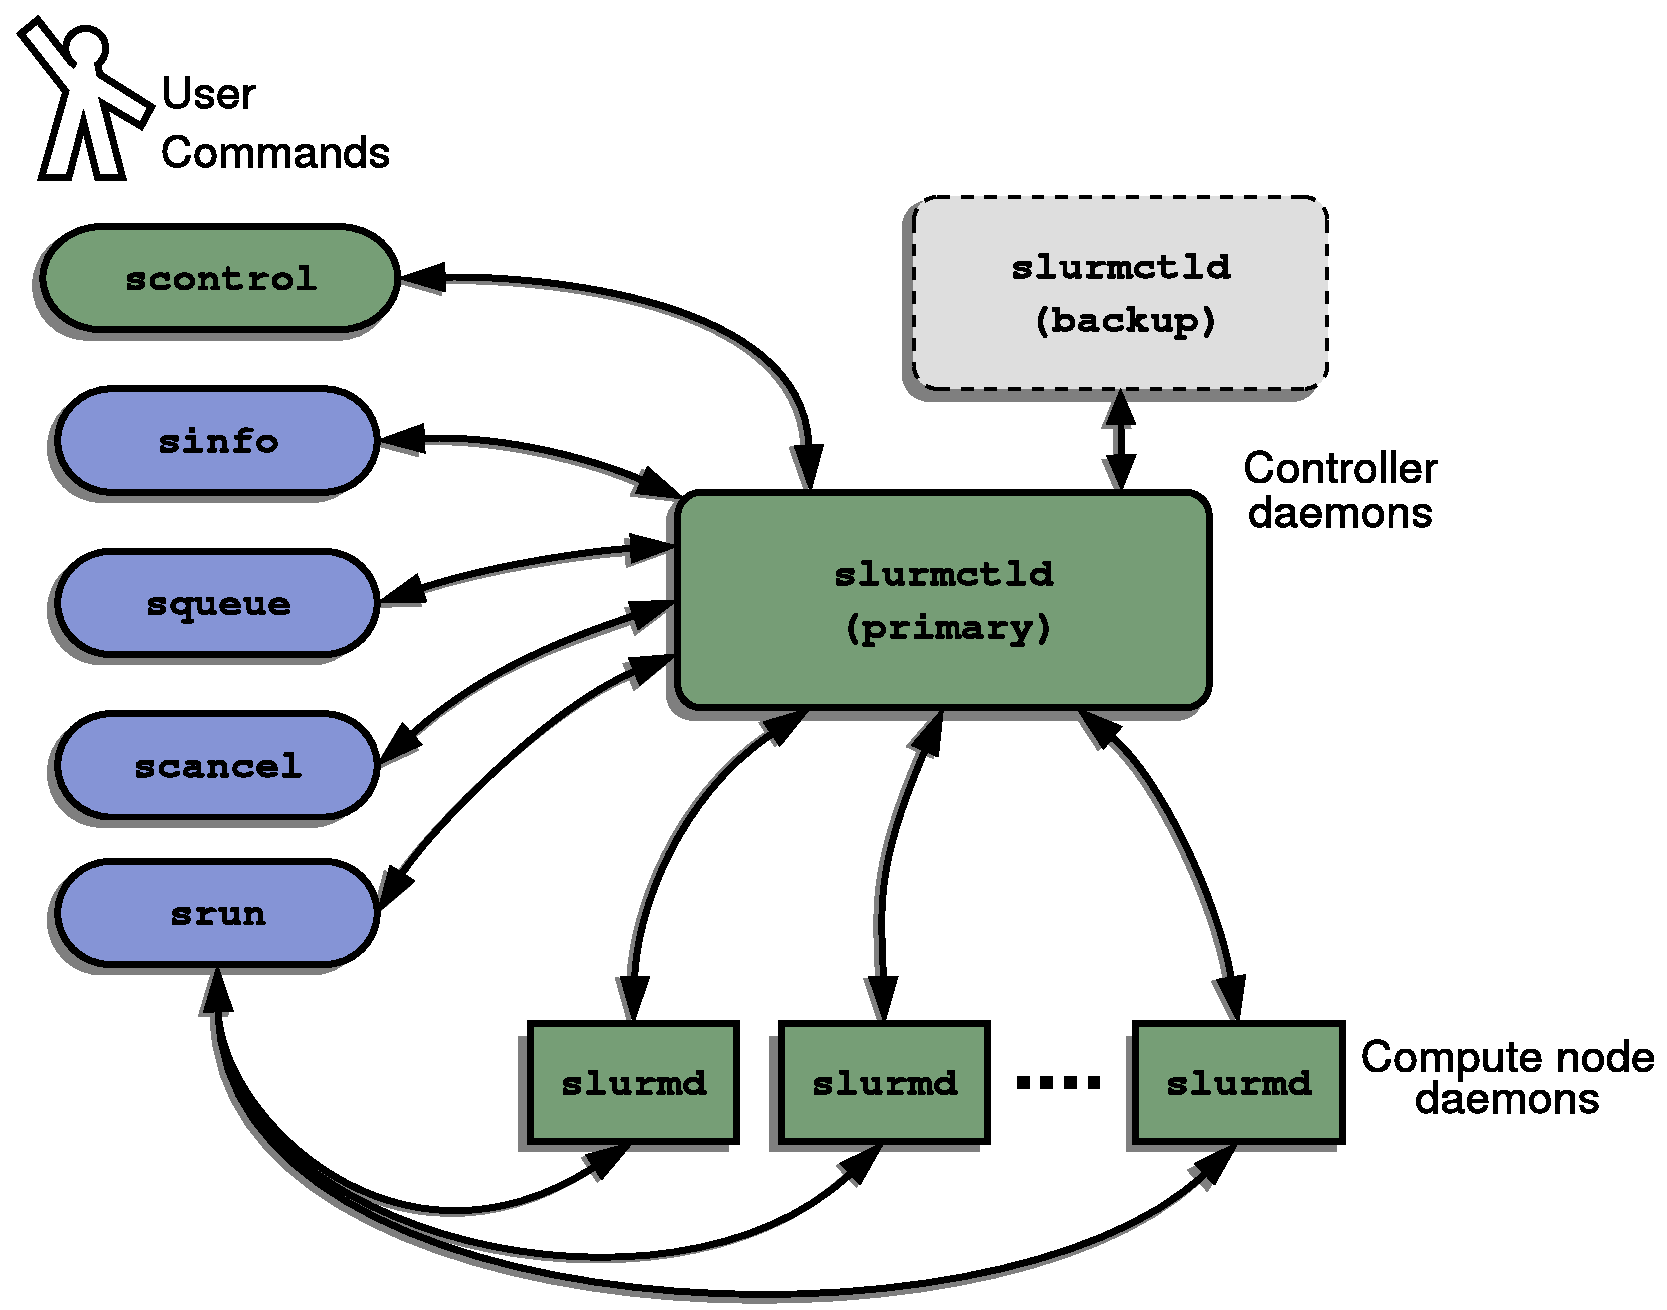
\epsfig{file=../figures/arch.eps,scale=0.35}}
\caption{\small SLURM architecture}
\label{arch}
\end{figure}

As shown in Figure~\ref{arch}, SLURM consists of a \slurmd\ daemon
running on each compute node, a central \slurmctld\ daemon running
on a management node (with optional fail-over twin), and five command
line utilities: {\tt srun}, {\tt scancel}, {\tt sinfo}, {\tt squeue},
and {\tt scontrol}, which can run anywhere in the cluster.

The entities managed by these SLURM daemons include {\em nodes}, the
compute resource in SLURM, {\em partitions}, which group nodes into
logical disjoint sets, {\em jobs}, or allocations of resources assigned
to a user for a specified amount of time, and {\em job steps}, which
are sets of (possibly parallel) tasks within a job.  Each job in the
priority-ordered queue is allocated nodes within a single partition.
Once an allocation request fails, no lower priority jobs for that
partition will be considered for a resource allocation.  Once a job is
assigned a set of nodes, the user is able to initiate parallel work in
the form of job steps in any configuration within the allocation. For
instance, a single job step may be started that utilizes all nodes
allocated to the job, or several job steps may independently use a
portion of the allocation.

\begin{figure}[tcb]
\centerline{\epsfig{file=../figures/entities.eps,scale=0.5}}
\caption{\small SLURM entities: nodes, partitions, jobs, and job steps}
\label{entities}
\end{figure}

Figure~\ref{entities} further illustrates the interrelation of these
entities as they are managed by SLURM by showing a group of
compute nodes split into two partitions. Partition 1 is running one job,
with one job step utilizing the full allocation of that job.  The job
in Partition 2 has only one job step using half of the original job
allocation.  That job might initiate additional job steps to utilize
the remaining nodes of its allocation.

\begin{figure}[tb]
\centerline{\epsfig{file=../figures/slurm-arch.eps,scale=0.5}}
\caption{SLURM architecture - subsystems}
\label{archdetail}
\end{figure}

Figure~\ref{archdetail} shows the subsystems that are implemented
within the \slurmd\ and \slurmctld\ daemons.  These subsystems are
explained in more detail below.

\subsection{Slurmd}

\slurmd\ is a multi-threaded daemon running on each compute node and
can be compared to a remote shell daemon: it reads the common SLURM
configuration file and saved state information, 
notifies the controller that it is active, waits
for work, executes the work, returns status, then waits for more work.
Because it initiates jobs for other users, it must run as user {\em root}.
It also asynchronously exchanges node and job status with {\tt slurmctld}.
The only job information it has at any given time pertains to its
currently executing jobs.  \slurmd\ has five major components:

\begin{itemize}
\item {\tt Machine and Job Status Services}:  Respond to controller
requests for machine and job state information and send asynchronous
reports of some state changes (e.g., \slurmd\ startup) to the controller.

\item {\tt Remote Execution}: Start, manage, and clean up after a set
of processes (typically belonging to a parallel job) as dictated by
the \slurmctld\ daemon or an \srun\ or \scancel\ command. Starting a
process may include executing a prolog program, setting process limits,
setting real and effective uid, establishing environment variables,
setting working directory, allocating interconnect resources, setting core
file paths, initializing stdio, and managing process groups. Terminating
a process may include terminating all members of a process group and
executing an epilog program.

\item {\tt Stream Copy Service}: Allow handling of stderr, stdout, and
stdin of remote tasks. Job input may be redirected 
from a single file or multiple files (one per task), an
\srun\ process, or /dev/null.  Job output may be saved into local files or
returned to the \srun\ command. Regardless of the location of stdout/err,
all job output is locally buffered to avoid blocking local tasks.

\item {\tt Job Control}: Allow asynchronous interaction with the Remote
Execution environment by propagating signals or explicit job termination
requests to any set of locally managed processes.

\end{itemize}

\subsection{Slurmctld}

Most SLURM state information exists in {\tt slurmctld}, also known as
the controller.  \slurmctld\ is multi-threaded with independent read
and write locks for the various data structures to enhance scalability.
When \slurmctld\ starts, it reads the SLURM configuration file and 
any previously saved state information.  Full controller state
information is written to disk periodically, with incremental changes
written to disk immediately for fault tolerance.  \slurmctld\ runs in
either master or standby mode, depending on the state of its fail-over
twin, if any.  \slurmctld\ need not execute as user {\em root}.  In fact,
it is recommended that a unique user entry be created for executing
\slurmctld\ and that user must be identified in the SLURM configuration
file as {\tt SlurmUser}.  \slurmctld\ has three major components:


\begin{itemize}
\item {\tt Node Manager}: Monitors the state of each node in the cluster.
It polls {\tt slurmd}s for status periodically and receives state
change notifications from \slurmd\ daemons asynchronously.  It ensures
that nodes have the prescribed configuration before being considered
available for use.

\item {\tt Partition Manager}: Groups nodes into non-overlapping sets
called partitions. Each partition can have associated with it
various job limits and access controls.  The Partition Manager also
allocates nodes to jobs based on node and partition states and
configurations. Requests to initiate jobs come from the Job Manager.
\scontrol\ may be used to administratively alter node and partition
configurations.

\item {\tt Job Manager}: Accepts user job requests and places pending jobs
in a priority-ordered queue.  The Job Manager is awakened on a periodic
basis and whenever there is a change in state that might permit a job to
begin running, such as job completion, job submission, partition {\em up}
transition, node {\em up} transition, etc.  The Job Manager then makes
a pass through the priority-ordered job queue. The highest priority
jobs for each partition are allocated resources as possible. As soon as
an allocation failure occurs for any partition, no lower-priority jobs
for that partition are considered for initiation.  After completing the
scheduling cycle, the Job Manager's scheduling thread sleeps.  Once a
job has been allocated resources, the Job Manager transfers necessary
state information to those nodes, permitting it to commence execution.
When the Job Manager detects that all nodes associated with a job
have completed their work, it initiates cleanup and performs another
scheduling cycle as described above.

\end{itemize}

\subsection{Command Line Utilities}

The command line utilities offer users access to remote execution and 
job control. They also permit administrators to dynamically change 
the system configuration. These commands use SLURM APIs that are 
directly available for more sophisticated applications.

\begin{itemize}
\item {\tt scancel}: Cancel a running or a pending job or job step,
subject to authentication and authorization. This command can also be
used to send an arbitrary signal to all processes on all nodes associated
with a job or job step.

\item {\tt scontrol}: Perform privileged administrative commands
such as bringing down a node or partition in preparation for maintenance.
Many \scontrol\ functions can only be executed by privileged users.

\item {\tt sinfo}: Display a summary of partition and node information.
An assortment of filtering and output format options are available.

\item {\tt squeue}: Display the queue of running and waiting jobs and/or
job steps. A wide assortment of filtering, sorting, and output format
options are available.

\item {\tt srun}: Allocate resources, submit jobs to the SLURM queue,
and initiate parallel tasks (job steps).  Every set of executing parallel
tasks has an associated \srun\ that initiated it and, if the \srun\
persists, manages it.  Jobs may be submitted for later execution
(e.g., batch), in which case \srun\ terminates after job submission.
Jobs may also be submitted for interactive execution, where \srun\ keeps
running to shepherd the running job. In this case, \srun\ negotiates
connections with remote {\tt slurmd}s for job initiation and to get
stdout and stderr, forward stdin,\footnote{\srun\ command line options
select the stdin handling method, such as broadcast to all tasks, or
send only to task 0.} and respond to signals from the user.  \srun\
may also be instructed to allocate a set of resources and spawn a shell
with access to those resources.

\end{itemize}

\subsection{Plugins}

In order to simplify the use of different infrastructures,
SLURM uses a general purpose plugin mechanism.  A SLURM plugin is a
dynamically linked code object that is loaded explicitly at run time
by the SLURM libraries.  A plugin provides a customized implementation
of a well-defined API connected to tasks such as authentication,
interconnect fabric, and task scheduling.  A common set of functions is defined
for use by all of the different infrastructures of a particular variety.
For example, the authentication plugin must define functions such as 
{\tt slurm\_auth\_create} to create a credential, {\tt slurm\_auth\_verify}
to verify a credential to approve or deny authentication, 
{\tt slurm\_auth\_get\_uid} to get the uid associated with a specific
credential, etc.  It also must define the data structure used, a plugin
type, a plugin version number, etc.  When a SLURM daemon is initiated, it
reads the configuration file to determine which of the available plugins
should be used.  For example {\em AuthType=auth/authd} says to use the
plugin for authd based authentication and {\em PluginDir=/usr/local/lib}
identifies the directory in which to find the plugin.

\subsection{Communications Layer}

SLURM presently uses Berkeley sockets for communications.  However,
we anticipate using the plugin mechanism to permit use of
other communications layers.  At LLNL we are using an Ethernet
for SLURM communications and the Quadrics Elan switch exclusively
for user applications.  The SLURM configuration file permits the
identification of each node's hostname as well as its name to be used
for communications.  In the case of a control machine known as {\em mcri}
to be communicated with using the name {\em emcri} (say to indicate an
Ethernet communications path), this is represented in the configuration
file as {\em ControlMachine=mcri ControlAddr=emcri}.  The name used for
communication is the same as the hostname unless otherwise specified.

Internal SLURM functions pack and unpack data structures in machine
independent format. We considered the use of XML style messages, but we
felt this would adversely impact performance (albeit slightly).  If XML
support is desired, it is straightforward to perform a translation and
use the SLURM APIs.


\subsection{Security}

SLURM has a simple security model: any user of the cluster may submit
parallel jobs to execute and cancel his own jobs.  Any user may view
SLURM configuration and state information.  Only privileged users
may modify the SLURM configuration, cancel any job, or perform other
restricted activities.  Privileged users in SLURM include the users 
{\em root} and {\em SlurmUser} (as defined in the SLURM configuration file).
If permission to modify SLURM configuration is required by others, set-uid
programs may be used to grant specific permissions to specific users.

\subsubsection{Communication Authentication.}

Historically, inter-node authentication has been accomplished via the use
of reserved ports and set-uid programs. In this scheme, daemons check the
source port of a request to ensure that it is less than a certain value
and thus only accessible by {\em root}. The communications over that
connection are then implicitly trusted.  Because reserved ports are a 
limited resource and set-uid programs are a possible security concern,
we have employed a credential-based authentication scheme that
does not depend on reserved ports. In this design, a SLURM authentication
credential is attached to every message and authoritatively verifies the
uid and gid of the message originator. Once recipients of SLURM messages
verify the validity of the authentication credential, they can use the uid
and gid from the credential as the authoritative identity of the sender.

The actual implementation of the SLURM authentication credential is
relegated to an ``auth'' plugin.  We presently have implemented three
functional authentication plugins: authd\cite{Authd2002}, 
Munge, and none.  The ``none'' authentication type employs a null
credential and is only suitable for testing and networks where security
is not a concern. Both the authd and Munge implementations employ
cryptography to generate a credential for the requesting user that
may then be authoritatively verified on any remote nodes. However, 
authd assumes a secure network and Munge does not.  Other authentication
implementations, such as a credential based on Kerberos, should be easy
to develop using the auth plugin API.

\subsubsection{Job Authentication.}

When resources are allocated to a user by the controller, a ``job step
credential'' is generated by combining the uid, job id, step id, the list
of resources allocated (nodes), and the credential lifetime and signing
the result with the \slurmctld\ private key.  This credential grants the
user access to allocated resources and removes the burden from \slurmd\
to contact the controller to verify requests to run processes. \slurmd\
verifies the signature on the credential against the controller's public
key and runs the user's request if the credential is valid.  Part of the
credential signature is also used to validate stdout, stdin,
and stderr connections from \slurmd\ to \srun .

\subsubsection{Authorization.}

Access to partitions may be restricted via a {\em RootOnly} flag.
If this flag is set, job submit or allocation requests to this partition
are only accepted if the effective uid originating the request is a
privileged user.  A privileged user may submit a job as any other user.
This may be used, for example, to provide specific external schedulers
with exclusive access to partitions.  Individual users will not be
permitted to directly submit jobs to such a partition, which would
prevent the external scheduler from effectively managing it.  Access to
partitions may also be restricted to users who are members of specific
Unix groups using a {\em AllowGroups} specification.

\subsection{Example: Executing a Batch Job}

In this example a user wishes to run a job in batch mode, in which \srun\
returns immediately and the job executes in the background when resources
are available.  The job is a two-node run of script containing {\em mping}, 
a simple MPI application.  The user submits the job:

\begin{verbatim}
srun --batch --nodes 2 --nprocs 2 mping.sh
\end{verbatim}
The script {\tt mping.sh} contains:
\begin{verbatim}
#!/bin/sh
srun hostname
srun mping 1 1048576
\end{verbatim}

The initial \srun\ command authenticates the user to the controller and
submits the job request.  The request includes the \srun\ environment,
current working directory, and command line option information. By
default, stdout and stderr are sent to files in the current working
directory and stdin is copied from {\tt /dev/null}.

The controller consults the Partition Manager to test whether the job 
will ever be able to run.  If the user has requested a non-existent partition,
a non-existent constraint, 
etc., the Partition Manager returns an error and the request is discarded.
The failure is reported to \srun\, which informs the user and exits, for 
example:
\begin{verbatim}
srun: error: Unable to allocate resources: Invalid partition name
\end{verbatim}

On successful submission, the controller assigns the job a unique 
{\em SLURM job id}, adds it to the job queue, and returns the job's
job id to \srun\, which reports this to user and exits, returning
success to the user's shell:

\begin{verbatim}
srun: jobid 42 submitted
\end{verbatim}

The controller awakens the Job Manager, which tries to run jobs starting
at the head of the priority ordered job queue.  It finds job {\em 42} and
makes a successful request to the Partition Manager to allocate two nodes
from the default (or requested) partition: {\em dev6} and {\em dev7}.

The Job Manager then sends a request to the \slurmd\ on the first
node in the job {\em dev6} to execute the script specified on the user's
command line.\footnote{Had the user specified an executable file rather
than a job script, an \srun\ program would be initiated on the first
node and \srun\ would initiate the executable with the desired task
distribution.}  The Job Manager also sends a copy of the environment,
current working directory, stdout and stderr location, along with other
options. Additional environment variables are appended to the user's
environment before it is sent to the remote \slurmd\ detailing the job's
resources, such as the SLURM job id ({\em 42}) and the allocated nodes
({\em dev[6-7]}).

The remote \slurmd\ establishes the new environment, executes a SLURM
prolog program (if one is configured) as user {\em root}, and executes
the job script (or command) as the submitting user. The \srun\ within
the job script detects that it is running with allocated resources from
the presence of a {\tt SLURM\_JOBID} environment variable. \srun\
connects to \slurmctld\ to request a job step to run on all nodes of
the current job. \slurmctld\ validates the request and replies with a
job step credential and switch resources. \srun\ then contacts {\tt slurmd}s
running on both {\em dev6} and {\em dev7}, passing the job step credential,
environment, current working directory, command path and arguments,
and interconnect information. The {\tt slurmd}s verify the valid job
step credential, connect stdout and stderr back to \srun , establish
the environment, and execute the command as the submitting user.

Unless instructed otherwise by the user, stdout and stderr are
copied to a file in the current working directory by \srun :
\begin{verbatim}
/path/to/cwd/slurm-42.out
\end{verbatim}

The user may examine output files at any time if they reside 
in a globally accessible directory. In this example
{\tt slurm-42.out} would  contain the output of the job script's two 
commands (hostname and mping):

\begin{verbatim}
dev6
dev7
  1 pinged   0:        1 bytes      5.38 uSec     0.19 MB/s                     
  1 pinged   0:        2 bytes      5.32 uSec     0.38 MB/s                     
  1 pinged   0:        4 bytes      5.27 uSec     0.76 MB/s                     
  1 pinged   0:        8 bytes      5.39 uSec     1.48 MB/s                     
  ...
  1 pinged   0:  1048576 bytes   4682.97 uSec   223.91 MB/s              
\end{verbatim}

When the tasks complete execution, \srun\ is notified by \slurmd\ of
each task's exit status. \srun\ reports job step completion to the Job
Manager and exits.  \slurmd\ detects when the job script terminates and
notifies the Job Manager of its exit status and begins cleanup.  The Job
Manager directs the {\tt slurmd}s formerly assigned to the job to run
the SLURM epilog program (if one is configured) as user {\em root}.
Finally, the Job Manager releases the resources allocated to job {\em 42} 
and updates the job status to {\em complete}. The record of a job's
existence is eventually purged.

\subsection{Example:  Executing an Interactive Job}

In this example a user wishes to run the same {\em mping} command 
in interactive mode, in which \srun\ blocks while the job executes 
and stdout/stderr of the job are copied onto stdout/stderr of {\tt srun}.
The user submits the job, this time without the {\tt batch} option:

\begin{verbatim}
srun --nodes 2 --nprocs 2 mping 1 1048576
\end{verbatim}

The \srun\ command authenticates the user to the controller and makes a
request for a resource allocation and job step. The Job Manager
responds with a list of nodes, a job step credential, and interconnect
resources on successful allocation. If resources are not immediately
available, the request terminates or blocks depending on user options.

If the request is successful, \srun\ forwards the job run request to
the assigned {\tt slurmd}s in the same manner as the \srun\ in the batch
job script. In this case, the user sees the program output on stdout of
{\tt srun}:

\begin{verbatim}
  1 pinged   0:        1 bytes      5.38 uSec     0.19 MB/s                     
  1 pinged   0:        2 bytes      5.32 uSec     0.38 MB/s                     
  1 pinged   0:        4 bytes      5.27 uSec     0.76 MB/s                     
  1 pinged   0:        8 bytes      5.39 uSec     1.48 MB/s                     
  ...
  1 pinged   0:  1048576 bytes   4682.97 uSec   223.91 MB/s              
\end{verbatim}

When the job terminates, \srun\ receives an EOF (End Of File) on each
stream and closes it, then receives the task exit status from each
{\tt slurmd}.  The \srun\ process notifies \slurmctld\ that the job is
complete and terminates. The controller contacts all {\tt slurmd}s allocated
to the terminating job and issues a request to run the SLURM epilog,
then releases the job's resources.

Most signals received by \srun\ while the job is executing are 
transparently forwarded to the remote tasks. SIGINT (generated by
Control-C) is a special case and only causes \srun\ to report 
remote task status unless two SIGINTs are received in rapid succession.
SIGQUIT (Control-$\backslash$) is another special case. SIGQUIT forces 
termination of the running job.

\section{Slurmctld Design}

\slurmctld\ is modular and multi-threaded with independent read and
write locks for the various data structures to enhance scalability.
The controller includes the following subsystems: Node Manager, Partition
Manager, and Job Manager.  Each of these subsystems is described in
detail below.

\subsection{Node Management}

The Node Manager monitors the state of nodes.  Node information monitored
includes:

\begin{itemize}
\item Count of processors on the node
\item Size of real memory on the node
\item Size of temporary disk storage
\item State of node (RUN, IDLE, DRAINED, etc.)
\item Weight (preference in being allocated work)
\item Feature (arbitrary description)
\item IP address
\end{itemize}

The SLURM administrator can specify a list of system node names using
a numeric range in the SLURM configuration file or in the SLURM tools
(e.g., ``{\em NodeName=linux[001-512] CPUs=4 RealMemory=1024 TmpDisk=4096 \linebreak
Weight=4 Feature=Linux}'').  These values for CPUs, RealMemory, and
TmpDisk are considered to be the minimal node configuration values
acceptable for the node to enter into service.  The \slurmd\ registers
whatever resources actually exist on the node, and this is recorded
by the Node Manager.  Actual node resources are checked on \slurmd\
initialization and periodically thereafter.  If a node registers with
less resources than configured, it is placed in DOWN state and
the event logged.  Otherwise, the actual resources reported are recorded
and possibly used as a basis for scheduling (e.g., if the node has more
RealMemory than recorded in the configuration file, the actual node
configuration may be used for determining suitability for any application;
alternately, the data in the configuration file may be used for possibly
improved scheduling performance).  Note the node name syntax with numeric
range permits even very large heterogeneous clusters to be described in
only a few lines.  In fact, a smaller number of unique configurations
can provide SLURM with greater efficiency in scheduling work.

{\em Weight} is used to order available nodes in assigning work to
them.  In a heterogeneous cluster, more capable nodes (e.g., larger memory
or faster processors) should be assigned a larger weight.  The units
are arbitrary and should reflect the relative value of each resource.
Pending jobs are assigned the least capable nodes (i.e., lowest weight)
that satisfy their requirements.  This tends to leave the more capable
nodes available for those jobs requiring those capabilities.

{\em Feature} is an arbitrary string describing the node, such as a
particular software package, file system, or processor speed.  While the
feature does not have a numeric value, one might include a numeric value
within the feature name (e.g., ``1200MHz'' or ``16GB\_Swap'').  If the
nodes on the cluster have disjoint features (e.g., different ``shared''
file systems), one should identify these as features (e.g., ``FS1'',
``FS2'', etc.).  Programs may then specify that all nodes allocated to
it should have the same feature, but that any of the specified features
are acceptable (e.g., ``$Feature=FS1|FS2|FS3$'' means the job should be
allocated nodes that all have the feature ``FS1'' or they all have feature
``FS2,'' etc.).

Node records are kept in an array with hash table lookup.  If nodes are
given names containing sequence numbers (e.g., ``lx01'', ``lx02'', etc.),
the hash table permits specific node records to be located very quickly;
therefore, this is our recommended naming convention for larger clusters.

An API is available to view any of this information and to update some
node information (e.g., state). APIs designed to return SLURM state
information permit the specification of a time stamp.  If the requested
data has not changed since the time stamp specified by the application,
the application's current information need not be updated.  The API
returns a brief ``No Change'' response rather than returning relatively
verbose state information.  Changes in node configurations (e.g., node
count, memory, etc.) or the nodes actually in the cluster should be
reflected in the SLURM configuration files. SLURM configuration may be
updated without disrupting any jobs.

\subsection{Partition Management}

The Partition Manager identifies groups of nodes to be used for execution
of user jobs. One might consider this the actual resource scheduling
component.  Data associated with a partition includes:

\begin{itemize}
\item Name
\item RootOnly flag to indicate that only users {\em root} or 
{\tt SlurmUser} may allocate resources in this partition (for any user)
\item List of associated nodes
\item State of partition (UP or DOWN)
\item Maximum time limit for any job
\item Minimum and maximum nodes allocated to any single job
\item List of groups permitted to use the partition (defaults to ALL)
\item Shared access (YES, NO, or FORCE)
\item Default partition (if no partition is specified in a job request)
\end{itemize}

It is possible to alter most of this data in real-time in order to affect
the scheduling of pending jobs (currently executing jobs would not be
affected).  This information is confined to the controller machine(s)
for better scalability.  It is used by the Job Manager (and possibly an
external scheduler), which either exist only on the control machine or
communicate only with the control machine.

The nodes in a partition may be designated for exclusive or non-exclusive
use by a job.  A {\tt shared} value of YES indicates that jobs may
share nodes on request.  A {\tt shared} value of NO indicates that
jobs are always given exclusive use of allocated nodes.  A {\tt shared}
value of FORCE indicates that jobs are never ensured exclusive
access to nodes, but SLURM may initiate multiple jobs on the nodes
for improved system utilization and responsiveness.  In this case,
job requests for exclusive node access are not honored.  Non-exclusive
access may negatively impact the performance of parallel jobs or cause
them to fail upon exhausting shared resources (e.g., memory or disk
space). However, shared resources may improve overall system utilization
and responsiveness. The proper support of shared resources, including
enforcement of limits on these resources, entails a substantial amount of
effort, which we are not presently planning to expend.  However, we have
designed SLURM so as to not preclude the addition of such a capability
at a later time if so desired.  Future enhancements could include
constraining jobs to a specific CPU count or memory size within a
node, which could be used to effectively space-share individual nodes.
The Partition Manager will allocate nodes to pending jobs on request
from the Job Manager.

Submitted jobs can specify desired partition, time limit, node count
(minimum and maximum), CPU count (minimum) task count, the need for
contiguous node assignment, and an explicit list of nodes to be included
and/or excluded in its allocation.  Nodes are selected so as to satisfy
all job requirements.  For example, a job requesting four CPUs and four
nodes will actually be allocated eight CPUs and four nodes in the case
of all nodes having two CPUs each.  The request may also indicate node
configuration constraints such as minimum real memory or CPUs per node,
required features, shared access, etc.  Overall there are 13 different
parameters that may identify resource requirements for a job.

Nodes are selected for possible assignment to a job based on the
job's configuration requirements (e.g., partition specification, minimum
memory, temporary disk space, features, node list, etc.).  The selection
is refined by determining which nodes are up and available for use.
Groups of nodes are then considered in order of weight, with the nodes
having the lowest {\em Weight} preferred.  Finally, the physical location
of the nodes is considered.

Bit maps are used to indicate which nodes are up, idle, associated
with each partition, and associated with each unique configuration.
This technique permits scheduling decisions to normally be made by
performing a small number of tests followed by fast bit map manipulations.
If so configured, a job's resource requirements would be compared with
the (relatively small number of) node configuration records, each of
which has an associated bit map. Usable node configuration bitmaps would
be ANDed with the selected partitions bit map ANDed with the UP node
bit map and possibly ANDed with the IDLE node bit map (this last test
depends on the desire to share resources).  This method can eliminate
tens of thousands of individual node configuration comparisons that 
would otherwise be required in large heterogeneous clusters.

The actual selection of nodes for allocation to a job is currently tuned
for the Quadrics interconnect.  This hardware supports hardware message
broadcast only if the nodes are contiguous.  If a job is not allocated
contiguous nodes, a slower software based multi-cast mechanism is used.
Jobs will be allocated continuous nodes to the extent possible (in
fact, contiguous node allocation may be specified as a requirement on
job submission).  If contiguous nodes cannot be allocated to a job, it
will be allocated resources from the minimum number of sets of contiguous
nodes possible.  If multiple sets of contiguous nodes can be allocated
to a job, the one that most closely fits the job's requirements will
be used.  This technique will leave the largest continuous sets of nodes
intact for jobs requiring them.

The Partition Manager builds a list of nodes to satisfy a job's request.
It also caches the IP addresses of each node and provides this information
to \srun\ at job initiation time for improved performance.

The failure of any node to respond to the Partition Manager only affects
jobs associated with that node.  In fact, a job may indicate it should
continue executing even if allocated nodes cease responding.  In this
case, the job needs to provide for its own fault tolerance.  All other
jobs and nodes in the cluster will continue to operate after a node
failure.  No additional work is allocated to the failed node, and it will
be pinged periodically to determine when it resumes responding. The node
may then be returned to service (depending on the {\tt ReturnToService}
parameter in the SLURM configuration).

\subsection{Configuration}

A single configuration file applies to all SLURM daemons and commands.
Most of this information is used only by the controller.  Only the
host and port information is referenced by most commands.  A sample
configuration file is shown in Table~\ref{sample_config}.


\begin{table}[t]
\begin{center}

\begin{tabular}[c]{c}
\\
\fbox{ 
   \begin{minipage}[c]{0.8\linewidth}
     {\tiny \verbatiminput{sample.config} } 
   \end{minipage} 
}
\\
\end{tabular}
\caption{Sample SLURM config file \label{sample_config}}
\end{center}
\end{table}



\subsection{Job Manager}

There are a multitude of parameters associated with each job, including:
\begin{itemize}
\item Job name
\item Uid
\item Job id
\item Working directory
\item Partition
\item Priority
\item Node constraints (processors, memory, features, etc.)
\end{itemize}

Job records have an associated hash table for rapidly locating 
specific records. They also have bit maps of requested and/or 
allocated nodes (as described above).

The core functions supported by the Job Manager include:
\begin{itemize}
\item Request resource (job may be queued)
\item Reset priority of a job
\item Status job (including node list, memory and CPU use data)
\item Signal job (send arbitrary signal to all processes associated 
      with a job)
\item Terminate job (remove all processes)
\item Change node count of running job (could fail if insufficient 
resources are available)
%\item Preempt/resume job  (future)
%\item Checkpoint/restart job (future)

\end{itemize}

Jobs are placed in a priority-ordered queue and allocated nodes as
selected by the Partition Manager.  SLURM implements a very simple default
scheduling algorithm, namely FIFO.  An attempt is made to schedule pending
jobs on a periodic basis and whenever any change in job, partition,
or node state might permit the scheduling of a job.

We are aware that this scheduling algorithm does not satisfy the needs
of many customers, and we provide the means for establishing other
scheduling algorithms. Before a newly arrived job is placed into the
queue, an external scheduler plugin assigns its initial priority.  
A plugin function is also called at the start of each scheduling
cycle to modify job or system state as desired.  SLURM APIs permit an
external entity to alter the priorities of jobs at any time and re-order
the queue as desired.  The Maui Scheduler \cite{Jackson2001,Maui2002}
is one example of an external scheduler suitable for use with SLURM.

LLNL uses DPCS \cite{DPCS2002} as SLURM's external scheduler. 
DPCS is a meta-scheduler with flexible scheduling algorithms that 
suit our needs well. 
It also provides the scalability required for this application.
DPCS maintains pending job state internally and only transfers the 
jobs to SLURM (or another underlying resources manager) only when 
they are to begin execution. 
By not transferring jobs to a particular resources manager earlier, 
jobs are assured of being initiated on the first resource satisfying 
their requirements, whether a Linux cluster with SLURM or an IBM SP 
with LoadLeveler (assuming a highly flexible application).
This mode of operation may also be suitable for computational grid 
schedulers.

In a future release, the Job Manager will collect resource consumption
information (CPU time used, CPU time allocated, and real memory used)
associated with a job from the \slurmd\ daemons.  Presently, only the
wall-clock run time of a job is monitored.  When a job approaches its
time limit (as defined by wall-clock execution time) or an imminent
system shutdown has been scheduled, the job is terminated.  The actual
termination process is to notify \slurmd\ daemons on nodes allocated
to the job of the termination request.  The \slurmd\ job termination
procedure, including job signaling, is described in Section~\ref{slurmd}.

One may think of a job as described above as an allocation of resources
rather than a collection of parallel tasks.  The job script executes
\srun\ commands to initiate the parallel tasks or ``job steps. '' The
job may include multiple job steps, executing sequentially and/or
concurrently either on separate or overlapping nodes.  Job steps have
associated with them specific nodes (some or all of those associated with
the job), tasks, and a task distribution (cyclic or block) over the nodes.

The management of job steps is considered a component of the Job Manager.
Supported job step functions include:
\begin{itemize}
\item Register job step
\item Get job step information
\item Run job step request
\item Signal job step
\end{itemize}

Job step information includes a list of nodes (entire set or subset of
those allocated to the job) and a credential used to bind communications
between the tasks across the interconnect. The \slurmctld\ constructs
this credential and sends it to the \srun\ initiating the job step.

\subsection{Fault Tolerance}
SLURM supports system level fault tolerance through the use of a secondary
or ``backup'' controller.  The backup controller, if one is configured,
periodically pings the primary controller.  Should the primary controller
cease responding, the backup loads state information from the last state
save and assumes control.  When the primary controller is returned to
service, it tells the backup controller to save state and terminate.
The primary then loads state and assumes control.

SLURM utilities and API users read the configuration file and initially try
to contact the primary controller.  Should that attempt fail, an attempt
is made to contact the backup controller before returning an error.

SLURM attempts to minimize the amount of time a node is unavailable
for work.  Nodes assigned to jobs are returned to the partition as
soon as they successfully clean up user processes and run the system
epilog.  In this manner,
those nodes that fail to successfully run the system epilog, or those
with unkillable user processes, are held out of the partition while
the remaining nodes are quickly returned to service.

SLURM considers neither the crash of a compute node nor termination
of \srun\ as a critical event for a job. Users may specify on a per-job
basis whether the crash of a compute node should result in the premature
termination of their job. Similarly, if the host on which \srun\ is
running crashes, the job continues execution and no output is lost.


\section{Slurmd Design}\label{slurmd}

The \slurmd\ daemon is a multi-threaded daemon for managing user jobs
and monitoring system state.  Upon initiation it reads the configuration
file, recovers any saved state, captures system state, 
attempts an initial connection to the SLURM
controller, and awaits requests.  It services requests for system state,
accounting information, job initiation, job state, job termination,
and job attachment. On the local node it offers an API to translate
local process ids into SLURM job id.

The most common action of \slurmd\ is to report system state on request.
Upon \slurmd\ startup and periodically thereafter, it gathers the
processor count, real memory size, and temporary disk space for the
node. Should those values change, the controller is notified.  In a
future release of SLURM, \slurmd\ will also capture CPU and real-memory and
virtual-memory consumption from the process table entries for uploading
to {\tt slurmctld}.

%FUTURE:  Another thread is
%created to capture CPU, real-memory and virtual-memory consumption from
%the process table entries.  Differences in resource utilization values
%from one process table snapshot to the next are accumulated. \slurmd\ 
%insures these accumulated values are not decremented if resource
%consumption for a user happens to decrease from snapshot to snapshot,
%which would simply reflect the termination of one or more processes.
%Both the real and virtual memory high-water marks are recorded and
%the integral of memory consumption (e.g. megabyte-hours).  Resource
%consumption is grouped by uid and SLURM job id (if any). Data
%is collected for system users ({\em root}, {\em ftp}, {\em ntp}, 
%etc.) as well as customer accounts. 
%The intent is to capture all resource use including
%kernel, idle and down time.  Upon request, the accumulated values are
%uploaded to \slurmctld\ and cleared.  

\slurmd\ accepts requests from \srun\ and \slurmctld\ to initiate
and terminate user jobs. The initiate job request contains such
information as real uid, effective uid, environment variables, working
directory, task numbers, job step credential, interconnect specifications and
authorization, core paths, SLURM job id, and the command line to execute.
System-specific programs can be executed on each allocated node prior
to the initiation of a user job and after the termination of a user
job (e.g., {\em Prolog} and {\em Epilog} in the configuration file).
These programs are executed as user {\em root} and can be used to
establish an appropriate environment for the user (e.g., permit logins,
disable logins, terminate orphan processes, etc.).  \slurmd\ executes
the prolog program, resets its session id, and then initiates the job
as requested. It records to disk the SLURM job id, session id, process
id associated with each task, and user associated with the job.  In the
event of \slurmd\ failure, this information is recovered from disk in
order to identify active jobs.

When \slurmd\ receives a job termination request from the SLURM
controller, it sends SIGTERM to all running tasks in the job,
waits for {\em KillWait} seconds (as specified in the configuration
file), then sends SIGKILL. If the processes do not terminate \slurmd\
notifies \slurmctld , which logs the event and sets the node's state
to DRAINED. After all processes have terminated, \slurmd\ executes the
configured epilog program, if any.

\section{Command Line Utilities}

\subsection{scancel}

\scancel\ terminates queued jobs or signals running jobs or job steps.
The default signal is SIGKILL, which indicates a request to terminate
the specified job or job step.  \scancel\ identifies the job(s) to
be signaled through user specification of the SLURM job id, job step id,
user name, partition name, and/or job state.  If a job id is supplied,
all job steps associated with the job are affected as well as the job
and its resource allocation.  If a job step id is supplied, only that
job step is affected.  \scancel\ can only be executed by the job's owner
or a privileged user.

\subsection{scontrol}

\scontrol\ is a tool meant for SLURM administration by user {\em root}. 
It provides the following capabilities:
\begin{itemize}
\item {\tt Shutdown}: Cause \slurmctld\ and \slurmd\ to save state 
and terminate.
\item {\tt Reconfigure}: Cause \slurmctld\ and \slurmd\ to reread the 
configuration file.
\item {\tt Ping}: Display the status of primary and backup \slurmctld\ daemons.
\item {\tt Show Configuration Parameters}: Display the values of general SLURM 
configuration parameters such as locations of files and values of timers.  
\item {\tt Show Job State}: Display the state information of a particular job 
or all jobs in the system.
\item {\tt Show Job Step State}: Display the state information of a particular 
job step or all job steps in the system.
\item {\tt Show Node State}: Display the state and configuration information 
of a particular node, a set of nodes (using numeric ranges syntax to 
identify their names), or all nodes.
\item {\tt Show Partition State}: Display the state and configuration 
information of a particular partition or all partitions.
\item {\tt Update Job State}: Update the state information of a particular job 
in the system. Note that not all state information can be changed in this 
fashion (e.g., the nodes allocated to a job).
\item {\tt Update Node State}: Update the state of a particular node. Note
that not all state information can be changed in this fashion (e.g., the
amount of memory configured on a node). In some cases, you may need
to modify the SLURM configuration file and cause it to be reread
using the ``Reconfigure'' command described above.  
\item {\tt Update Partition State}: Update the state of a partition
node. Note that not all state information can be changed in this fashion
(e.g., the default partition). In some cases, you may need to modify
the SLURM configuration file and cause it to be reread using the
``Reconfigure'' command described above.  
\end{itemize}

\subsection{squeue}

\squeue\ reports the state of SLURM jobs.  It can filter these
jobs input specification of job state (RUN, PENDING, etc.), job id,
user name, job name, etc.  If no specification is supplied, the state of
all pending and running jobs is reported. 
\squeue\ also has a variety of sorting and output options.

\subsection{sinfo}

\sinfo\ reports the state of SLURM partitions and nodes.  By default,
it reports a summary of partition state with node counts and a summary
of the configuration of those nodes.  A variety of sorting and 
output formatting options exist.

\subsection{srun}

\srun\ is the user interface to accessing resources managed by SLURM.
Users may utilize \srun\ to allocate resources, submit batch jobs,
run jobs interactively, attach to currently running jobs, or launch a
set of parallel tasks (job step) for a running job. \srun\ supports a
full range of options to specify job constraints and characteristics,
for example minimum real memory, temporary disk space, and CPUs per node,
as well as time limits, stdin/stdout/stderr handling, signal handling,
and working directory for job.  The full range of options is detailed
in Table~\ref{srun_opts}.

\begin{table}[!tb]
\begin{center}
  \begin{tabular}[t]{lcl}
   \hhline{---}
      Option & Arg Type & Description \\
   \hhline{---}
      {\em attach}	   & string & attach \srun\ to a running job	      \\

      {\em allocate}	   & boolean& allocate nodes only		      \\
      {\em batch}	   & boolean& submit a batch script to job queue      \\
      {\em cddir}	   & string & working directory of remote processes   \\
      {\em constraint}     & string & arbitrary feature constraints	      \\
      {\em contiguous}	   & boolean& allocate contiguous nodes only	      \\
      {\em cpus-per-task } & number & number of CPUs needed per process      \\
      {\em distribution}   & string & distribution method for processes (block$|$cyclic) \\
      {\em error}	   & string & location of stderr redirection	      \\
      {\em exclude}	   & string & do not allocate from a specific set of hosts \\
      {\em immediate}	   & boolean& exit if resources are not immediately available  \\
      {\em input}	   & string & location of stdin redirection	      \\
      {\em join}	   & string & join existing \srun\ to collect output of a running job \\
      {\em job-name}	   & string & name of job 			      \\
      {\em label}	   & boolean& prepend task number to lines of stdout/err \\
      {\em mem}		   & number & minimum amount of real memory per node  \\
      {\em mincpus} 	   & number & minimum number of CPUs per node         \\
%     {\em no-allocate}    & boolean& do not allocate nodes, SlurmUser only   \\
      {\em no-kill}	   & boolean& don't kill job if allocated nodes fail  \\
      {\em nodelist}	   & string & request a specific set of hosts	      \\
      {\em nodes}	   & numbers& minimum and maximum number of nodes on which to run \\
      {\em ntasks}         & number & number of tasks to run     	      \\
      {\em output}         & string & location of stdout redirection	      \\
      {\em overcommit}     & boolean& allow more than 1 process per CPU	      \\
      {\em partition}	   & string & partition name in which to run          \\
      {\em share}	   & boolean& allow nodes to be shared with other jobs \\
%     {\em slurmd-debug}   & number & get slurmd error message at this level of detail \\
      {\em threads}        & number & run with this number of communication threads \\
      {\em time}           & number & wall-clock time limit in minutes        \\
      {\em tmp}	           & number & minimum amount of temporary disk space  \\
      {\em verbose}	   & boolean& verbose operation			      \\
      {\em version}	   & boolean& print \srun\ version and exit	      \\
      {\em wait}           & number & seconds to wait after first task end before killing job \\
   \hhline{---}
  \end{tabular}
\caption{\label{srun_opts} List of \srun\ user options}
\end{center}
\end{table}

The \srun\ utility can run in four different modes: {\em interactive},
in which the \srun\ process remains resident in the user's session,
manages stdout/stderr/stdin, and forwards signals to the remote tasks;
{\em batch}, in which \srun\ submits a job script to the SLURM queue for
later execution; {\em allocate}, in which \srun\ requests resources from
the SLURM controller and spawns a shell with access to those resources;
{\em attach}, in which \srun\ attaches to a currently
running job and displays stdout/stderr in real time from the remote
tasks.  

% FUTURE:
% An interactive job may also be forced into the background with a special
% control sequence typed at the user's terminal.  Output from the running
% job is subsequently redirected to files in the current working directory
% and stdin is copied from {\tt /dev/null}. A backgrounded job may be
% reattached to a user's terminal at a later time by running
% \begin{verbatim}
%   srun --attach <jobid>
% \end{verbatim}
% at any time, though the remote \srun\ is not terminated as the result
% of an attach.

\section{Job Initiation Design}

There are three modes in which jobs may be run by users under SLURM. The
first and most simple mode is {\em interactive} mode, in which stdout and
stderr are displayed on the user's terminal in real time, and stdin and
signals may be forwarded from the  terminal transparently to the remote
tasks. The second mode is {\em batch} or {\em queued} mode, in which the job is
queued until the request for resources can be satisfied, at which time the
job is run by SLURM as the submitting user. In the third mode,{\em allocate} 
mode, a job is allocated to the requesting user, under which the user may
manually run job steps via a script or in a sub-shell spawned by \srun .

\begin{figure}[tb]
\centerline{\epsfig{file=../figures/connections.eps,scale=0.4}}
\caption{\small Job initiation connections overview. 1. \srun\ connects to 
         \slurmctld\ requesting resources. 2. \slurmctld\ issues a response,
	 with list of nodes and job step credential. 3. \srun\ opens a listen
	 port for job IO connections, then sends a run job step
	 request to \slurmd . 4. \slurmd initiates job step and connects
	 back to \srun\ for stdout/err }
\label{connections}
\end{figure}

Figure~\ref{connections} shows a high-level depiction of the connections
that occur between SLURM components during a general interactive
job startup.  \srun\ requests a resource allocation and job step
initiation from the {\tt slurmctld}, which responds with the job id,
list of allocated nodes, job step credential, etc.  if the request is granted,
\srun\ then initializes a listen port for stdio connections and connects
to the {\tt slurmd}s on the allocated nodes requesting that the remote
processes be initiated. The {\tt slurmd}s begin execution of the tasks and
connect back to \srun\ for stdout and stderr. This process and other
initiation modes are described in more detail below.

\subsection{Interactive Job Initiation}

\begin{figure}[tb]
\centerline{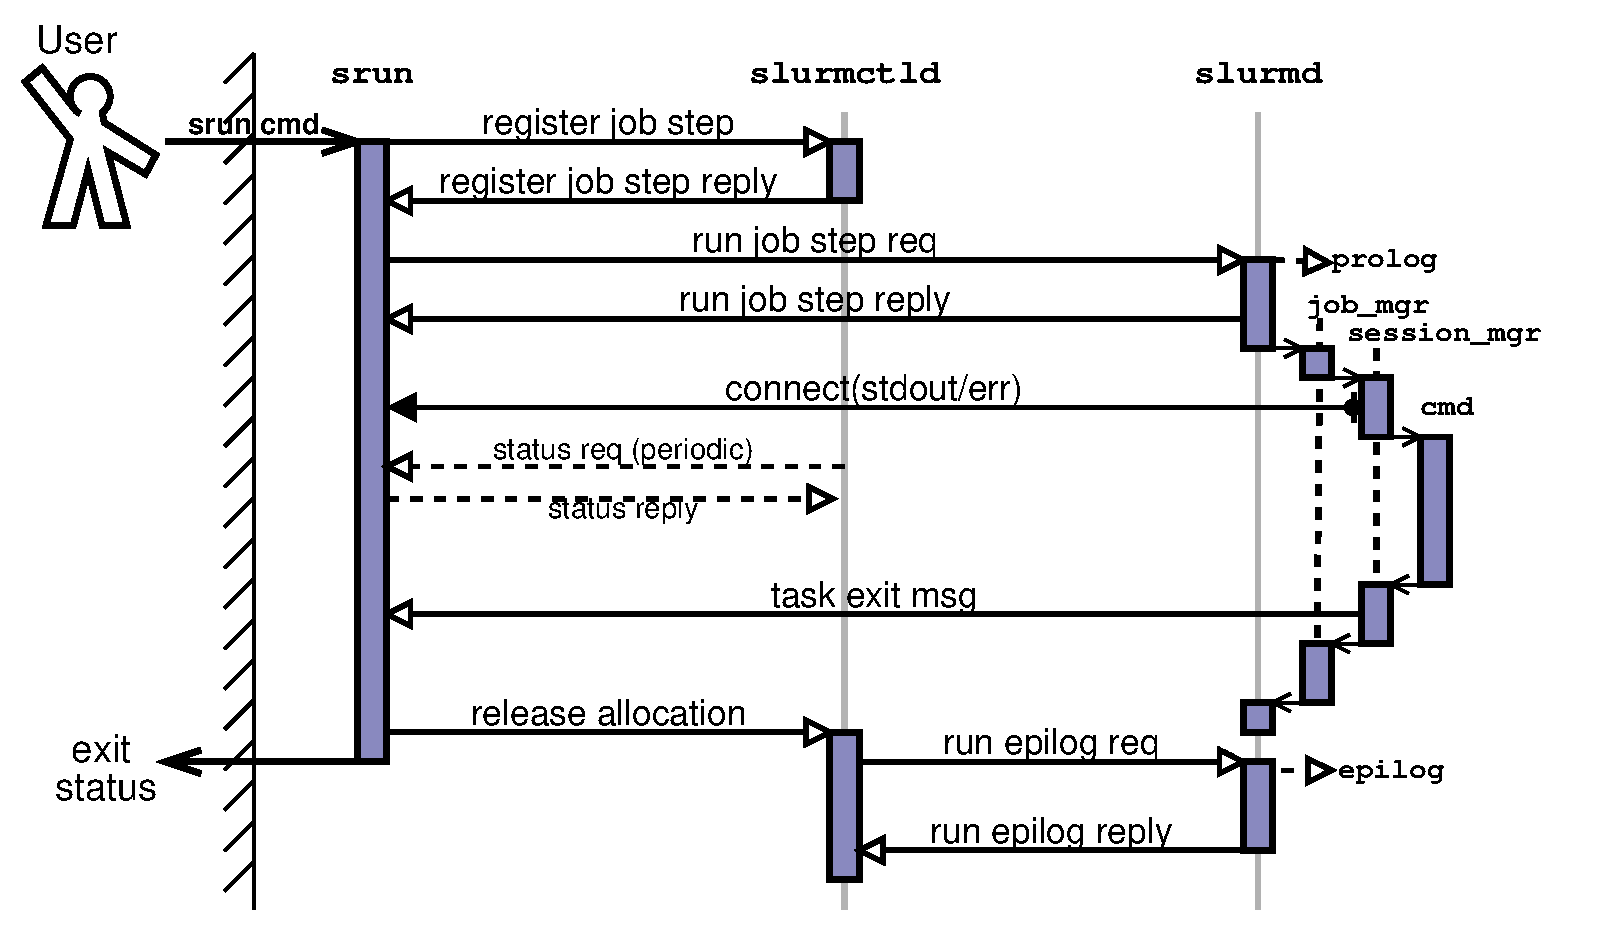
\epsfig{file=../figures/interactive-job-init.eps,scale=0.45} }
\caption{\small Interactive job initiation. \srun\ simultaneously allocates
	 nodes and a job step from \slurmctld\ then sends a run request to all
	 {\tt slurmd}s in job. Dashed arrows indicate a periodic request that
	 may or may not occur during the lifetime of the job}
\label{init-interactive}
\end{figure}

Interactive job initiation is shown in
Figure~\ref{init-interactive}.  The process begins with a user invoking
\srun\ in interactive mode.  In Figure~\ref{init-interactive}, the user
has requested an interactive run of the executable ``{\tt cmd}'' in the
default partition.

After processing command line options, \srun\ sends a message to
\slurmctld\ requesting a resource allocation and a job step initiation.
This message simultaneously requests an allocation (or job) and a job
step.  \srun\ waits for a reply from {\tt slurmctld}, which may not come
instantly if the user has requested that \srun\ block until resources are
available.  When resources are available for the user's job, \slurmctld\
replies with a job step credential, list of nodes that were allocated,
cpus per node, and so on. \srun\ then sends a message each \slurmd\ on
the allocated nodes requesting that a job step be initiated. 
The \slurmd\ daemons verify that the job is valid using the forwarded job 
step credential and then respond to \srun .

Each \slurmd\ invokes a job manager process to handle the request, which
in turn invokes a session manager process that initializes the session for
the job step. An IO thread is created in the job manager that connects
all tasks' IO back to a port opened by \srun\ for stdout and stderr.
Once stdout and stderr have successfully been connected, the task thread
takes the necessary steps to initiate the user's executable on the node,
initializing environment, current working directory, and interconnect
resources if needed.

Each \slurmd\ forks a copy of itself that is responsible for the job
step on this node. This local job manager process then creates an
IO thread that initializes stdout, stdin, and stderr streams for each
local task and connects these streams to the remote \srun . Meanwhile,
the job manager forks a session manager process that initializes
the session becomes the requesting user and invokes the user's processes.

As user processes exit, their exit codes are collected, aggregated when
possible, and sent back to \srun\ in the form of a task exit message.
Once all tasks have exited, the session manager exits, and the job
manager process waits for the IO thread to complete, then exits.
The \srun\ process either waits for all tasks to exit, or attempts to
clean up the remaining processes some time after the first task exits
(based on user option).  Regardless, once all tasks are finished,
\srun\ sends a message to the \slurmctld\ releasing the allocated nodes,
then exits with an appropriate exit status.

When the \slurmctld\ receives notification that \srun\ no longer needs
the allocated nodes, it issues a request for the epilog to be run on
each of the {\tt slurmd}s in the allocation. As {\tt slurmd}s report that the
epilog ran successfully, the nodes are returned to the partition.

\subsection{Queued (Batch) Job Initiation}

\begin{figure}[tb]
\centerline{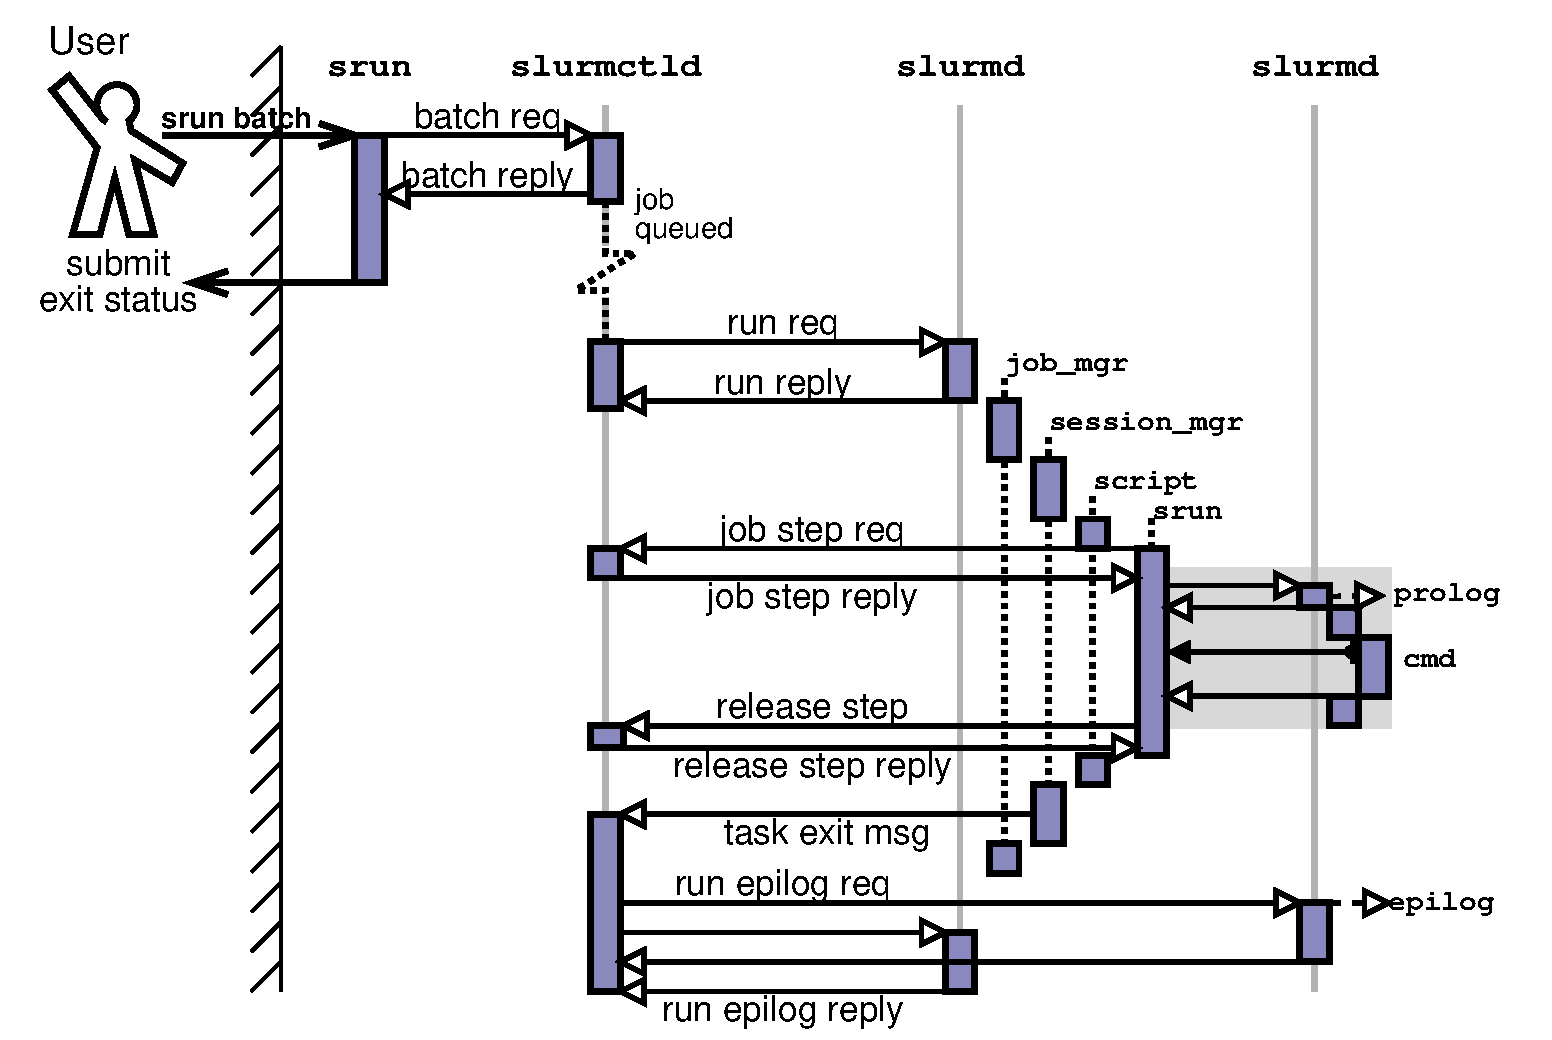
\epsfig{file=../figures/queued-job-init.eps,scale=0.45} }
\caption{\small Queued job initiation. 
         \slurmctld\ initiates the user's job as a batch script on one node. 
	 Batch script contains an \srun\ call that initiates parallel tasks 
	 after instantiating job step with controller. The shaded region is 
	 a compressed representation and is shown in more detail in the 
	 interactive diagram (Figure~\ref{init-interactive})}
\label{init-batch}
\end{figure}

Figure~\ref{init-batch} shows the initiation of a queued job in
SLURM.  The user invokes \srun\ in batch mode by supplying the {\tt --batch}
option to \srun . Once user options are processed, \srun\ sends a batch
job request to \slurmctld\ that identifies the stdin, stdout and stderr file 
names for the job, current working directory, environment, requested 
number of nodes, etc. 
The \slurmctld\ queues the request in its priority-ordered queue.

Once the resources are available and the job has a high enough priority, \linebreak
\slurmctld\ allocates the resources to the job and contacts the first node
of the allocation requesting that the user job be started. In this case,
the job may either be another invocation of \srun\ or a job script
including invocations of \srun . The \slurmd\ on
the remote node responds to the run request, initiating the job manager,
session manager, and user script. An \srun\ executed from within the script
detects that it has access to an allocation and initiates a job step on
some or all of the nodes within the job.

Once the job step is complete, the \srun\ in the job script notifies
the \slurmctld\, and terminates. The job script continues executing and
may initiate further job steps. Once the job script completes, the task
thread running the job script collects the exit status and sends a task
exit message to the \slurmctld . The \slurmctld\ notes that the job
is complete and requests that the job epilog be run on all nodes that
were allocated.  As the {\tt slurmd}s respond with successful completion
of the epilog, the nodes are returned to the partition.

\subsection{Allocate Mode Initiation}

\begin{figure}[tb]
\centerline{\epsfig{file=../figures/allocate-init.eps,scale=0.45} }
\caption{\small Job initiation in allocate mode. Resources are allocated and
         \srun\ spawns a shell with access to the resources. When user runs 
	 an \srun\ from within the shell, the a job step is initiated under
	 the allocation}
\label{init-allocate}
\end{figure}

In allocate mode, the user wishes to allocate a job and interactively run
job steps under that allocation. The process of initiation in this mode
is shown in Figure~\ref{init-allocate}. The invoked \srun\ sends
an allocate request to \slurmctld , which, if resources are available,
responds with a list of nodes allocated, job id, etc. The \srun\ process
spawns a shell on the user's terminal with access to the allocation,
then waits for the shell to exit (at which time the job is considered
complete).

An \srun\ initiated within the allocate sub-shell recognizes that
it is running under an allocation and therefore already within a
job. Provided with no other arguments, \srun\ started in this manner
initiates a job step on all nodes within the current job. 

% Maybe later: 
%
% However, the user may select a subset of these nodes implicitly by using
% the \srun\ {\tt --nodes} option, or explicitly by specifying a relative
% nodelist ( {\tt --nodelist=[0-5]} ).

An \srun\ executed from the sub-shell reads the environment and user
options, then notifies the controller that it is starting a job step under
the current job. The \slurmctld\ registers the job step and responds
with a job step credential. \srun\ then initiates the job step using the same
general method as for interactive job initiation.

When the user exits the allocate sub-shell, the original \srun\ receives
exit status, notifies \slurmctld\ that the job is complete, and exits.
The controller runs the epilog on each of the allocated nodes, returning
nodes to the partition as they successfully complete the epilog.

%
% Information in this section seems like it should be some place else
% (Some of it is incorrect as well)
% -mark
%
%\section{Infrastructure}
%
%The state of \slurmctld\ is written periodically to disk for fault
%tolerance.  SLURM daemons are initiated via {\tt inittab} using the {\tt
%respawn} option to insure their continuous execution.  If the control
%machine itself becomes inoperative, its functions can easily be moved in
%an automated fashion to another node. In fact, the computers designated

%as both primary and backup control machine can easily be relocated as
%needed without loss of the workload by changing the configuration file
%and restarting all SLURM daemons.
%
%The {\tt syslog} tools are used for logging purposes and take advantage

%of the severity level parameter.
%
%Direct use of the Elan interconnect is provided a version of MPI developed
%and supported by Quadrics. SLURM supports this version of MPI with no
%modifications.
%
%SLURM supports the TotalView debugger\cite{Etnus2002}.  This requires
%\srun\ to not only maintain a list of nodes used by each job step, but
%also a list of process ids on each node corresponding the application's
%tasks.

\section{Results}

\begin{figure}[htb]
\centerline{\epsfig{file=../figures/times.eps}}
\caption{Time to execute /bin/hostname with various node counts}
\label{timing}
\end{figure}

We were able to perform some SLURM tests on a 1000-node cluster 
in November 2002. Some development was still underway at that time 
and tuning had not been performed. The results for executing the 
program {\em /bin/hostname} on two tasks per node and various node 
counts are shown in Figure~\ref{timing}. We found SLURM performance 
to be comparable to the
Quadrics Resource Management System (RMS) \cite{Quadrics2002} for all
job sizes and about 80 times faster than IBM LoadLeveler\cite{LL2002}
at tested job sizes.

\section{Future Plans}

SLURM begin production use on LLNL Linux clusters in March 2003 
and is available from our web site\cite{SLURM2003}. 

While SLURM is able to manage 1000 nodes without difficulty using
sockets and Ethernet, we are reviewing other communication mechanisms
that may offer improved scalability.  One possible alternative
is STORM \cite{STORM2001}.  STORM uses the cluster interconnect
and Network Interface Cards to provide high-speed communications,
including a broadcast capability.  STORM only supports the Quadrics
Elan interconnnect at present, but it does offer the promise of improved
performance and scalability.

Looking ahead, we anticipate adding support for additional 
interconnects (InfiniBand and the IBM
Blue Gene \cite{BlueGene2002} system\footnote{Blue Gene has a different
interconnect than any supported by SLURM and a 3-D topography with
restrictive allocation constraints.}).  We anticipate adding a job
preempt/resume capability to the next release of SLURM.  This will
provide an external scheduler the infrastructure required to perform gang
scheduling.  We also anticipate adding a checkpoint/restart capability at
some time in the future ,and we plan to support changing the node count
associated with running jobs (as needed for MPI2).  Recording resource
use by each parallel job is planned for a future release.

\section{Acknowledgments}

SLURM is jointly developed by LLNL and Linux NetworX.
Contributers to SLURM development include:
\begin{itemize}
\item Jay Windley of Linux NetworX for his development of the plugin 
mechanism and work on the security components
\item Joey Ekstrom for his work developing the user tools
\item Kevin Tew for his work developing the communications infrastructure
\item Jim Garlick for his development of the Quadrics Elan interface and 
technical guidance
\item Gregg Hommes, Bob Wood, and Phil Eckert for their help designing the 
SLURM APIs
\item Mark Seager and Greg Tomaschke for their support of this project
\item Chris Dunlap for technical guidance
\item David Jackson of Linux NetworX for technical guidance
\item Fabrizio Petrini of Los Alamos National Laboratory for his work to 
integrate SLURM with STORM communications 
\end{itemize}

%\appendix
%\newpage
%\section{Glossary}
%
%\begin{description}
%\item[Authd]    User authentication mechanism
%\item[DCE]	Distributed Computing Environment
%\item[DFS]	Distributed File System (part of DCE)
%\item[DPCS]	Distributed Production Control System, a meta-batch system 
%		and resource manager developed by LLNL
%\item[Globus]	Grid scheduling infrastructure
%\item[Kerberos]	Authentication mechanism
%\item[LoadLeveler] IBM's parallel job management system
%\item[LLNL]	Lawrence Livermore National Laboratory
%\item[Munge]   User authentication mechanism developed by LLNL
%\item[NQS]	Network Queuing System (a batch system)
%\item[RMS]	Quadrics' Resource Management System
%\item[TotalView] Etnus' debugger
%\end{description}

% make the bibliography
\bibliographystyle{unsrt}
\bibliography{project}

% make the back cover page
\makeLLNLBackCover
\end{document}
